\section{Zuordnung der Molekülschwingungen zu den Ramanlinien \& Diskussion}
\subsection{Vorwissen}
Um den Ramanlinien nun eine Molekülschwingung zuzuordnen ist etwas Vorarbeit nötig.\\
Je symmetrischer die Schwingung des Moleküls ist, desto kleiner ist ihr Depolarisationsgrad (Bei einer symmetrischen Schwingung ist der Polarisationsgrad gleich null) \citep[vgl.][]{Polgrad1}.
Je kleiner der Depolarisationsgrad der Linie ist, desto polarisierter ist diese im Spektrum.\\
Des weiteren wird zwischen Valenz- und Deformationsschwingungen unterschieden.
Bei Ersteren verändern sich die Bindungslängen, was mehr Energie braucht \citep[vgl.][]{Valenz}.
Bei Deformationsschwingungen hingegen ändern sich nur die Bindungswinkel, was mit geringerem Energieaufwand stattfinden kann und sich mit einer kleineren Wellenzahl zeigt \citep[vgl.][]{Deformation}.\\
Nun folg noch aus der klassischen Mechanik, dass ein harmonischer Oszillator mit einer hohen Masse langsamer schwingt als einer mit einer kleinen.
Deswegen hat man bei hohen Massen kleine Wellenzahlen.\\

Komplett symmetrische fünfatomige Moleküle der Form $CY_4$, wie $CCl_4$ können folgende Normalschwingungen haben:
\begin{figure}[h]
    \centering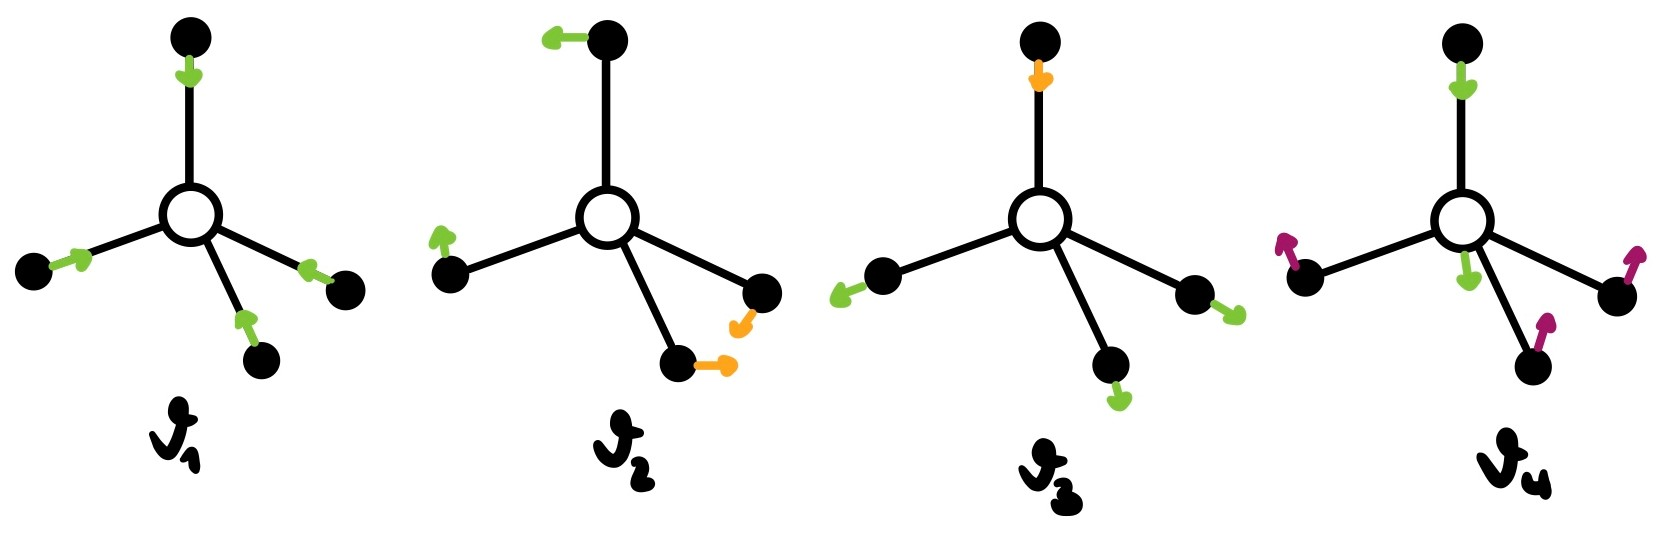
\includegraphics[width=0.6\textwidth]{Moleküle/3bearbeitet.jpg}
    \caption{Normalschwingungen für symmetrische fünfatomige Moleküle}
\end{figure}\\
Fünfatomige Moleküle der Form $CXY_3$, wie der Rest den von uns vermessenen Proben, können folgende Normalschwingungen haben:
\begin{figure}[h]
    \centering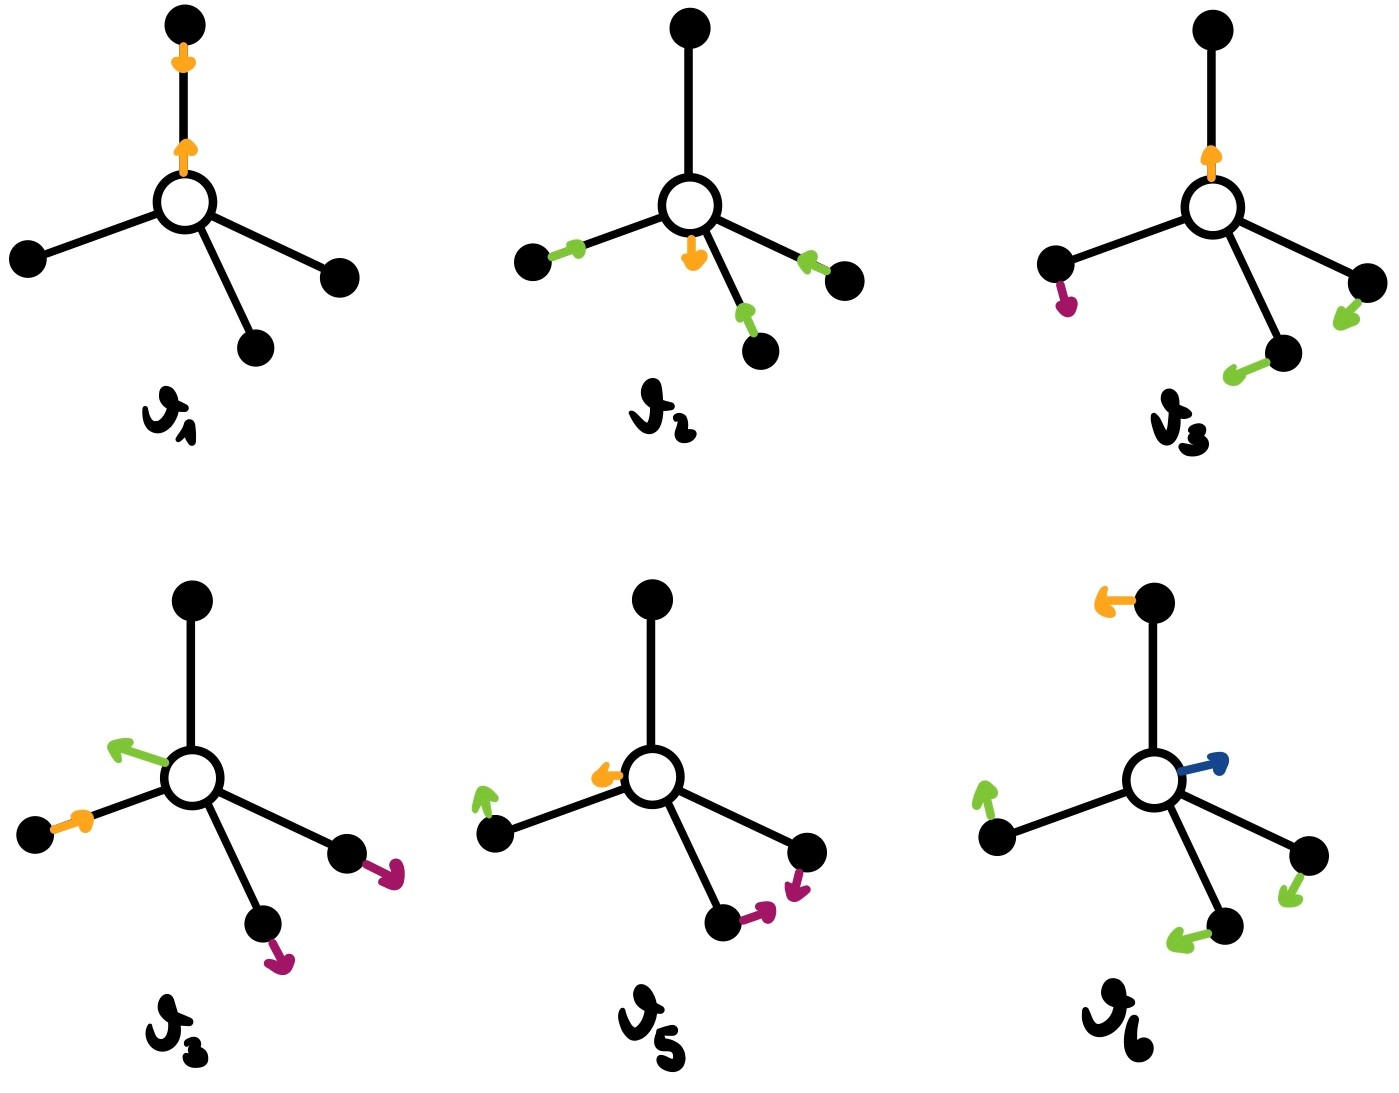
\includegraphics[width=0.55\textwidth]{Moleküle/6bearbeitet.jpg}
    \caption{Normalschwingungen für nicht symmetrische fünfatomige Moleküle}
\end{figure}\newpage
\subsection{Zuordnung von Molekülschwingungen zu den gemessenen Linien}
\subsubsection{CCl$_4$}
Bei $CCl_4$ ist die am stärksten polarisierte Schwingung, jene mit dem Literaturwert $\tilde{\nu}=458,4\,\text{cm}^{-1}$.
Deswegen handelt es sich bei dieser Schwingung um die symmetrischste der Normalschwingungen, also die Valenzschwingung $\nu_1$.\\
Die Schwingung mit der größten Wellenzahlen, $\tilde{\nu}=762,0\,\text{cm}^{-1}$, muss auch eine Valenzschwingung sein.
Daher kommt hier nur die Normalschwingung $\nu_3$ in Frage.\\
Die restlichen beiden Linien sind Deformationsschwingungen.
Die Schwingung mit der höheren Energie, $\tilde{\nu}=314,0\,\text{cm}^{-1}$ ist der Normalschwingung $\nu_4$ zugeordnet, da diese an einer Bindung ein Teil einer Valenzschwingung ausführt.\\
Somit folgt nun, dass der Linie $\tilde{\nu}=217,9\,\text{cm}^{-1}$ die Normalschwingung $\nu_2$ zugeordnet werden kann.\\
Zusammengefasst folgt:
\begin{table}[h]
    \centering\begin{tabular}{c|c}
        Normalschwingung & $(\nu_{CCl_4})_l$ (cm$^{-1}$)\\\hline
        $\nu_1$&458,4\\
        $\nu_2$&217,9\\
        $\nu_3$&762,0\\
        $\nu_4$&314,0      
    \end{tabular}
    \caption{Zuordnung der Normalschwingungen zu den dazugehörigen Literaturwerten}
\end{table}
\subsubsection{CHCl$_3$,CDCl$_3$,CHBr$_3$}
Durch die Symmetriebrechung entstehen zwei weitere Normalschwingung.\\
Es werden nun die Linien anhand von $CHCl_3$ den einzelnen Schwingungen zugeordnet und dann die Wellenzahlen von den anderen beiden Proben übernommen.\\
Bei $CHCl_3$ sind zwei polarisierte Linien erkennbar, nämlich $\tilde{\nu}=365,9\,\text{cm}^{-1}$ und $\tilde{\nu}=668,3\,\text{cm}^{-1}$.
Dieser werden den zwei symmetrischsten Normalschwingungen $\nu_2$ und $\nu_3$ zugeordnet.
Die höhere Wellenzahl wird der Normalschwingung $\nu_2$ zugeordnet, da diese mehr Valenzschwingung besitzt als die Normalschwingung $\nu_3$.
Die Normalschwingung $\nu_3$ wird also der niedrigeren Wellenzahl zugeordnet, da es eine Deformationsschwingung ist.\\
Die Schwingung mit der höchsten Wellenzahl $\tilde{\nu}_l=3018,9\text{cm}^{-1}$ wird der Normalschwingung $\nu_1$ zugeordnet, da es sich hierbei um eine Valenzschwingung der C-H Achse handelt (kleine Masse $\to$ hohe Wellenzahl).\\
Die Linie $\tilde{\nu}_l=1215,6\text{cm}^{-1}$ kann man der Normalschwingung $\nu_6$ zuzuordnen, da hier wieder das H-Atom mitbewegt wird, was eine hohe Wellenzahl zur Folge hat.\\
Der Normalschwingung $\nu_4$ ordnet man die Linie $\tilde{\nu}_l=761,2\text{cm}^{-1}$ zu, da hier das Molekül eine Valenzschwingung ohne das H-Atom ausführt.\\
Somit bleibt nur noch für die Linie $\tilde{\nu}_l=260,0\text{cm}^{-1}$ die Normalschwingung $\nu_5$ übrig, was auch sinnig ist, da hier eine Deformationsschwingung ohne das H-Atom ausgeführt wird.\newpage
Zusammengefasst folgt:
\begin{table}[h]
    \centering\begin{tabular}{c|ccc}
        Normalschwingung & $(\nu_{CHCl_3})_l$ (cm$^{-1}$)& $(\nu_{CDCl_3})_l$ (cm$^{-1}$)& $(\nu_{CHBr_3})_l$ (cm$^{-1}$)\\\hline
        $\nu_1$&3018,9&2250,0&3023,0\\
        $\nu_2$&668,3&650,8&538,5\\
        $\nu_3$&365,9&366,5&222,3\\
        $\nu_4$&761,2&737,6&656,0\\
        $\nu_5$&260,0&262,0&153,8\\
        $\nu_6$&1215,6&908,3&1142,0
    \end{tabular}
    \caption{Zuordnung der Normalschwingungen zu den unsymmetrischen Molekülen mit den entsprechenden Literaturwerten}
\end{table}\\
Beim Austausch von Chlor zu Brom ($CHCl_3\leftrightarrow CHBr_3$) oder Wasserstoff zu Deuterium\\
($CHCl_3\leftrightarrow CDCl_3$)ändert sich die Zuordnung der Normalschwingungen nicht.
Er werden zwar die einzelnen Linien 'herumgeschoben' aufgrund des Massenunterschieds.\\
Zum Beispiel sind die Wellenzahlen für die Linien mit Brom geringer, als die mit Chlor, da Brom um einiges schwerer ist als Chlor.
Besonders deutlich wird es wenn man sich die Normalschwingung $\nu_1$ für Wasserstoff und Deuterium anschaut.
Da Deuterium doppelt so schwer wie Wasserstoff ist, ist die Schwingungslinien von Deuterium viel kleiner als die von Wasserstoff (ca. nur ein Viertel davon).
